We present here images that can be interesting but are not fundamental for the report.
\begin{figure}[h]
    \centering
    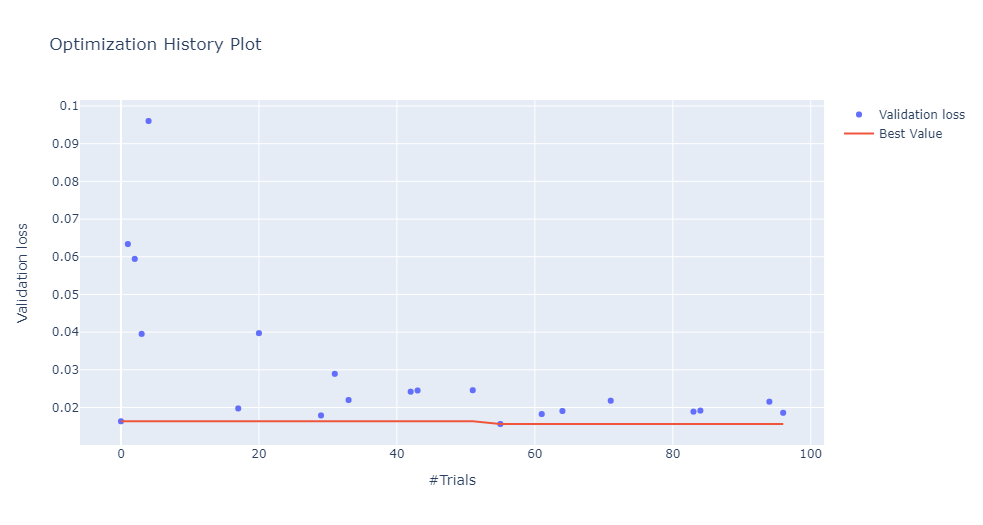
\includegraphics[width=0.8\textwidth]{Images/Optimization.png}
    \caption{Optimization trend of the validation loss. On the y-axis we report the final validation loss, while on the x-axis the trial number.
        The red line represents the evolution of the best score.}
    \label{fig:opt}
\end{figure}

\begin{figure}[h]
    \centering
    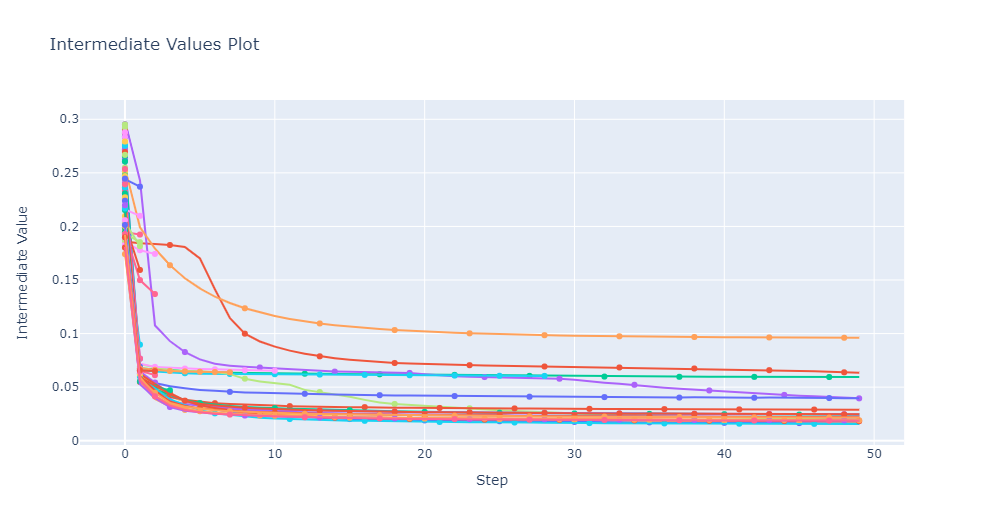
\includegraphics[width=0.8\textwidth]{Images/Losses.png}
    \caption{Evolution of the validation loss. While some trial is pruned at the beginning for a poor performance we can observe 
        that the validation loss converges quite quickly.}
    \label{fig:losses}
\end{figure}

\begin{figure}[h]
    \centering
    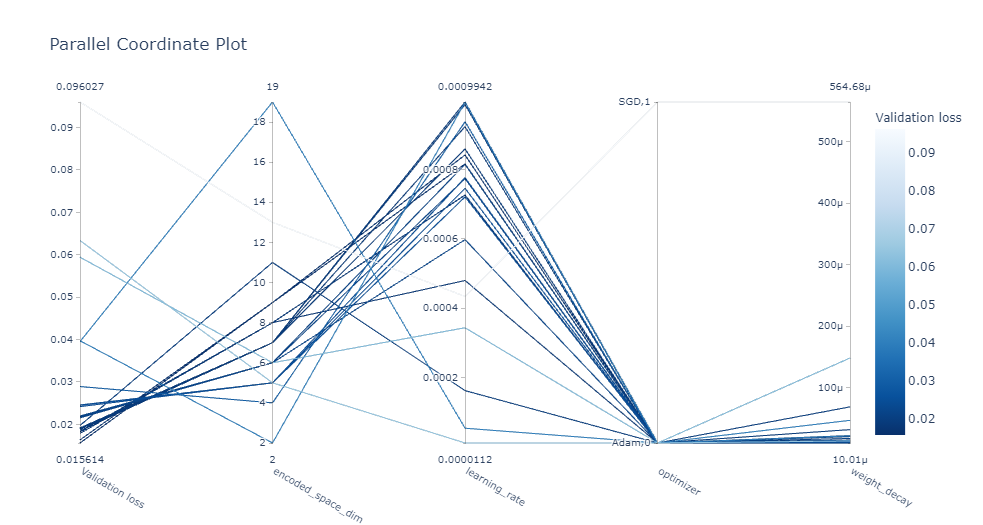
\includegraphics[width=0.8\textwidth]{Images/Hyperparams.png}
    \caption{Visual representation of the used hyperparameters, where the color of the line connecting the parameters used in a single 
    trial is related to the validation loss as shown in the colorbar. We can observe that the stochastic gradient descent is not 
    performing well.}
    \label{fig:hyper}
\end{figure}

\begin{figure}[h]
    \centering
    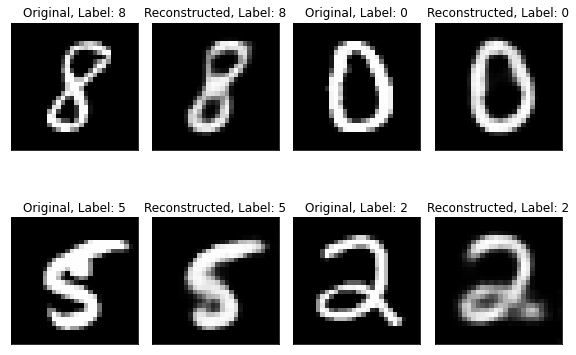
\includegraphics[width=0.6\textwidth]{Images/reconstr_im.png}
    \caption{Reconstruction of the Autoencoder with optimized hyperparameters}
    \label{fig:rec}
\end{figure}

\begin{figure}[h]
    \centering
    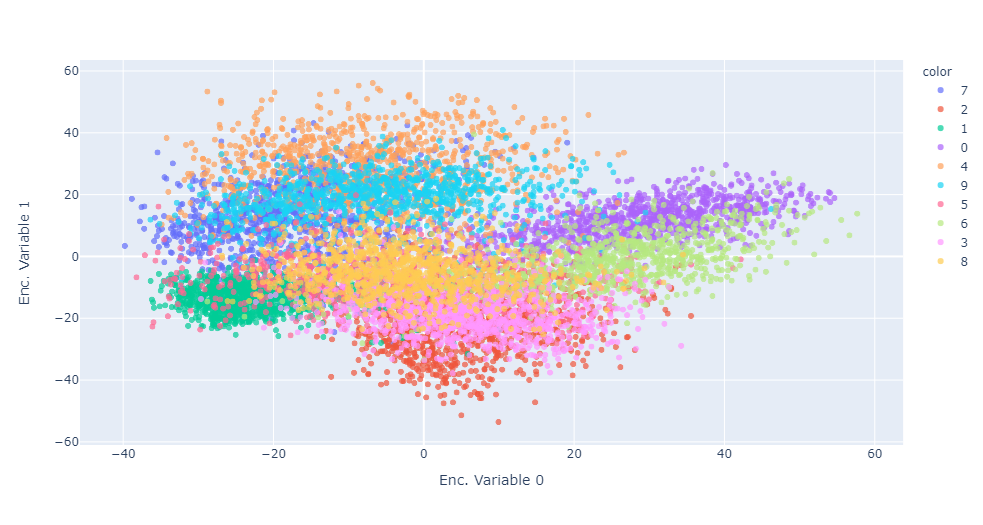
\includegraphics[width=0.8\textwidth]{Images/autoenc_PCA.png}
    \caption{Encoded space with dimensionality reduced with PCA for the classical Autoencoder, using as points the test set.}
    \label{fig:aut_PCA}
\end{figure}

\begin{figure}[h]
    \centering
    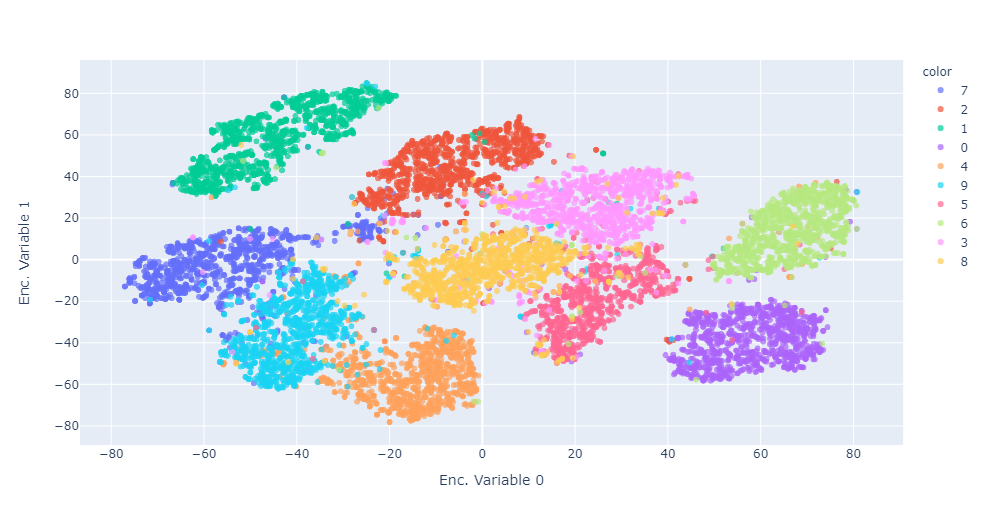
\includegraphics[width=0.8\textwidth]{Images/autoenc_tsne.png}
    \caption{Encoded space with dimensionality reduced with PCA for the classical Autoencoder, using as points the test set.}
    \label{fig:aut_TSNE}
\end{figure}

\begin{figure}[h]
    \centering
    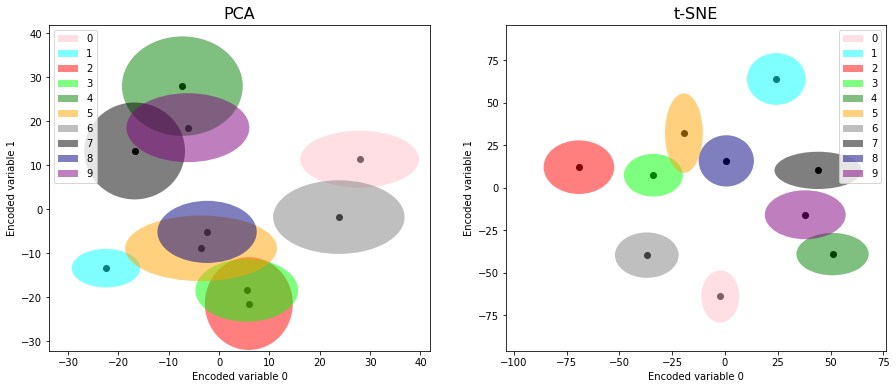
\includegraphics[width=0.8\textwidth]{Images/autoenc.png}
    \caption{Encoded space with dimensionality reduction for the classical autoencoder, where the center of the ellipse is the average position of a given digit, 
    while the ellipse represents its standard deviation along the two different coordinates.}
    \label{fig:dim_red_aut}
\end{figure}

\begin{figure}[h]
    \centering
    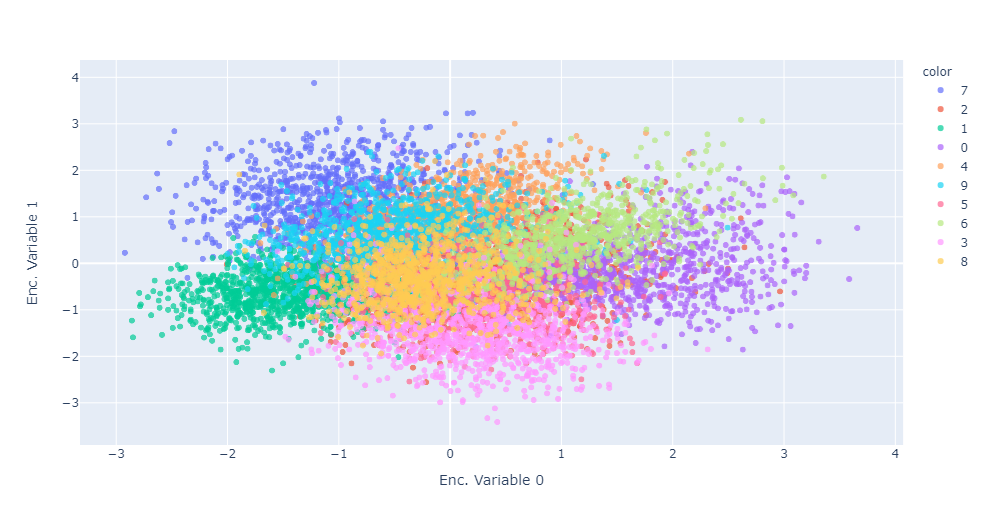
\includegraphics[width=0.8\textwidth]{Images/VAE_PCA.png}
    \caption{Encoded space with dimensionality reduced with PCA for the Variational Autoencoder, using as points the test set.}
    \label{fig:vae_PCA}
\end{figure}

\begin{figure}[h]
    \centering
    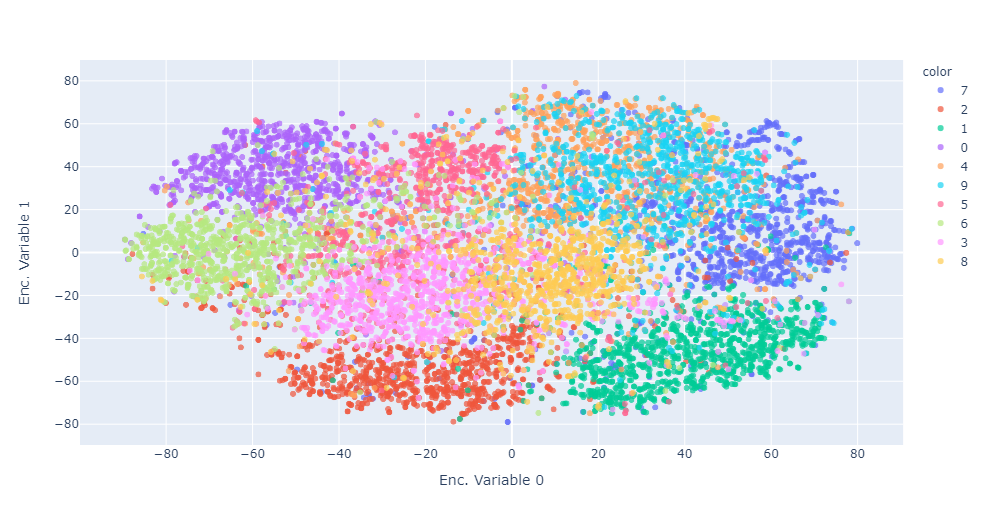
\includegraphics[width=0.8\textwidth]{Images/VAE_tsne.png}
    \caption{Encoded space with dimensionality reduced with PCA for the Variational Autoencoder, using as points the test set.}
    \label{fig:vae_TSNE}
\end{figure}

\begin{figure}[h]
    \centering
    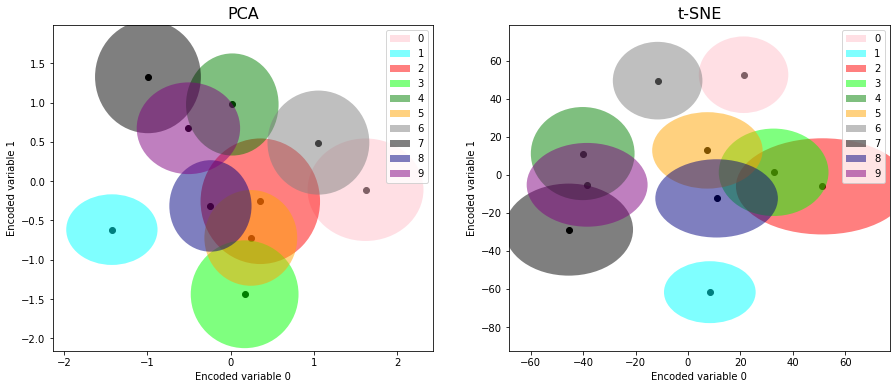
\includegraphics[width=0.8\textwidth]{Images/VAE.png}
    \caption{Encoded space with dimensionality reduction for the Variational autoencoder, where the center of the ellipse is the average position of a given digit, 
    while the ellipse represents its standard deviation along the two different coordinates.}
    \label{fig:dim_red_vae}
\end{figure}

\begin{figure}[h]
    \centering
    \begin{minipage}[t]{0.48\textwidth}
        \centering
        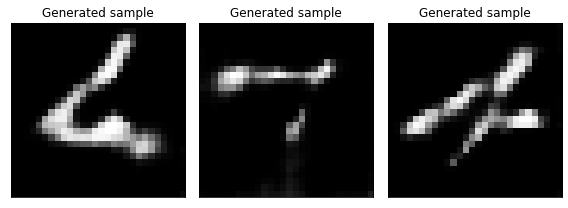
\includegraphics[width=0.98\textwidth]{Images/autoenc_generated.png}
        \caption{Images generated by sampling the classical autencoder using a normal ditribution.}
        \label{fig:gen_aut}
    \end{minipage}\hfill
    \begin{minipage}[t]{0.48\textwidth}
        \centering
        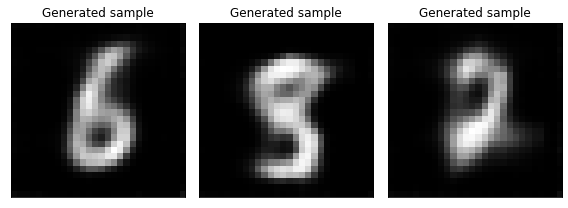
\includegraphics[width=0.98\textwidth]{Images/vae_generated.png}
        \caption{Images generated by sampling the variational autencoder using a normal ditribution.}
        \label{fig:gen_vae}
    \end{minipage}
\end{figure}
